% !Mode:: "TeX:UTF-8"%確保文檔utf-8編碼
\documentclass{standalone}
\usepackage{tikz}
\usetikzlibrary{calc}
\usepackage{pgfplots}
\pgfplotsset{compat=newest}
\begin{document}
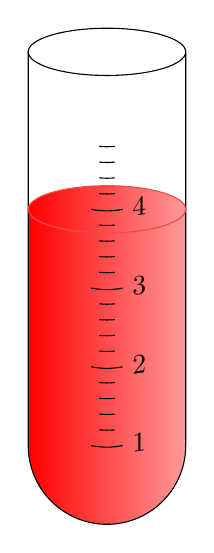
\begin{tikzpicture}
\shade[left color=red,right color=red!40] 
    (-1,-2)--(-1,-5) arc (180:360:1)  -- (1,-2) arc (0:180:1 and 0.3);
\draw (0,0) ellipse (1 and .3);
\draw (-1,0)--(-1,-5) arc (180:360:1) --(1,-5) -- (1,0);
\draw[red!90!black!70] (0,-2) ellipse (1 and .3);

\foreach \y/\x in {-5/1,-4/2,-3/3,-2/4}
    {
    \draw (-0.2,\y) to[bend right=10](0.2,\y) node[right,yslant=0.15](\x){\x};

    \foreach \z in {0.2,0.4,0.6,0.8}
       \draw ($(-0.1,\z) + (0,\y)$)to[bend right=5]($(0.1,\z)+(0,\y)$);
    };
    
\end{tikzpicture}
\end{document}